\section{Statistics}\label{sec:statistics}

Every science starts from a hypothesis to be tested. The task is to make a statement if the proposed hypothesis agrees or disagrees with observed data, to either accept or reject it against the null-hypothesis. The metric at hand to do so is the p-value that arises within hypothesis testing. 

For exactly this task high energy physicists have developed a framework based on likelihood statistics tailored for counting experiments. This section begins to lay out the fundamentals of the approach and then goes to the hands on implementation of its use. The following is based on \citep{cowan2011asymptotic,behnke2013data,pyhf_intro}.

\subsection{Building the likelihood}
As we are dealing with a counting experiment the tool at hand are histograms $\bm{n}=(n_1,...,n_N)$. It can be modeled with a set of parameters divided into so called parameters of interest, here only the signal strength $\mu$, and nuisance parameters $\bm{\Theta}$, that basically serve to give the model flexibility to fit the observations. The bin heights (counts) can then be expressed in terms of the amount of signal $s_i(\bm{\Theta})$ and background $b_i(\bm{\Theta})$ in them. The expectation value of the $n_i$ is then
\begin{equation} \label{eq:n_i}
    \langle n_i(\mu,\bm{\Theta})\rangle = \mu s_i(\bm{\Theta}) +b_i(\bm{\Theta}).
\end{equation}
The model can be further constrained with auxiliary histograms $\bm{a}=(a_1,...,a_M)$ with bin height
\begin{equation} \label{eq:a_i}
    \langle a_i(\bm{\Theta}) \rangle = u_i(\bm{\Theta}).
\end{equation}
As we are expecting the bin counts to occur with a constant mean rate and independent of time compared to the last event each follows a Poisson distribution
\begin{equation}\label{eq:poisson}
    \frac{r^k e^{-r}}{k!}.
\end{equation}
$r$ is the expected rate of occurrences, which translates as our prediction, whereas $k$ are the actual measured occurrences. From this a likelihood $L(\bm{x})$ can be built, which is just a probability under a given set of parameters $\bm{x}$. Accounting for all the bins by multiplying them together yields
\begin{equation}
    L(\mu,\bm{\Theta})=
    \prod_{j=1}^N \frac{(\mu s_j + b_j)^{n_j}}{n_j !} e^{-(\mu s_j + b_j)}
    \prod_{k=1}^M \frac{u_k^{a_k}}{a_k!} e^{-u_k}.
\end{equation}
To test for a hypothesized value of $\mu$ we consider the so called profile likelihood ratio that reduces the dependence to one parameter of interest $\mu$
\begin{equation}
\lambda(\mu)=
    \frac{L(\mu,\hat{\hat{\bm{\Theta}}})}
    {L(\hat{\mu},\hat{\bm{\Theta}})}
\end{equation}
The denominator is the unconditional maximum likelihood estimation so that $\hat{\mu}$ and $\hat{\bm{\Theta}}$ both are free to vary to maximize $L$. Whereas the numerator is the found maximum likelihood conditioned on some chosen $\mu$ and the set of found nuisance parameters $\hat{\hat{\bm{\Theta}}}$ that maximize the likelihood. This definition gives $0 \leq \lambda \leq 1$. For a $\lambda \sim 1$ the hypothesized value of $\mu$ shows good agreement to the Poissonian model.

\subsection{From test statistic to p-value}   
Transforming this into a test statistic $t_{\mu}$ is practical to calculate p-values
\begin{equation}
    t_{\mu}=-2\log \lambda(\mu).
\end{equation}
This translates as $t_{\mu} \rightarrow 0$ as good agreement, $t_{\mu} \rightarrow \infty$ as bad agreement to the model. A p-value can then be calculated from the probability density function of $t_\mu$: pdf$(t_\mu) = f(t_\mu \mid \mu)$
\begin{equation}\label{eq:p-value}
    p_\mu = \int_{t_{\mu ,obs}}^{\infty} 
    f(t_\mu \mid \mu) \mathrm{d}t_\mu
\end{equation}
$t_{\mu ,obs}$ is the test statistic $t_\mu$ evaluated at the observed data. This is like plugging into the Poisson distributions the same values for $r$ as for $k$ in eq. \ref{eq:poisson} \footnote{The subindex $\mu$ for the observation in $t_{\mu ,obs}$ can be a bit misleading because plugging in actually drops the dependency on $\mu$.}. Just like a probability density function for a standard normal distribution, intuitively the pdf is just how probable the test statistic $t_\mu$ is under a fixed value of the signal strength (how often it occurs compared to all other values $t_\mu$ can be). This particular form is handy because there exist approximations for $f(t_\mu \mid \mu)$ (for details see \citep{cowan2011asymptotic}). Figure \ref{fig:test_stat_example} illustrates the different steps as a sketch. One caveat here is that this assumes $\mu$ can also take negative values which of course is not the intended goal here. But considering the correct limiting cases one can construct test statistics accordingly (\citep{cowan2011asymptotic} for details). In the scientific community a widely accepted threshold to accept an alternative hypothesis over the null hypothesis is for a p-value of 0.05. 
\begin{figure}
    \centering
    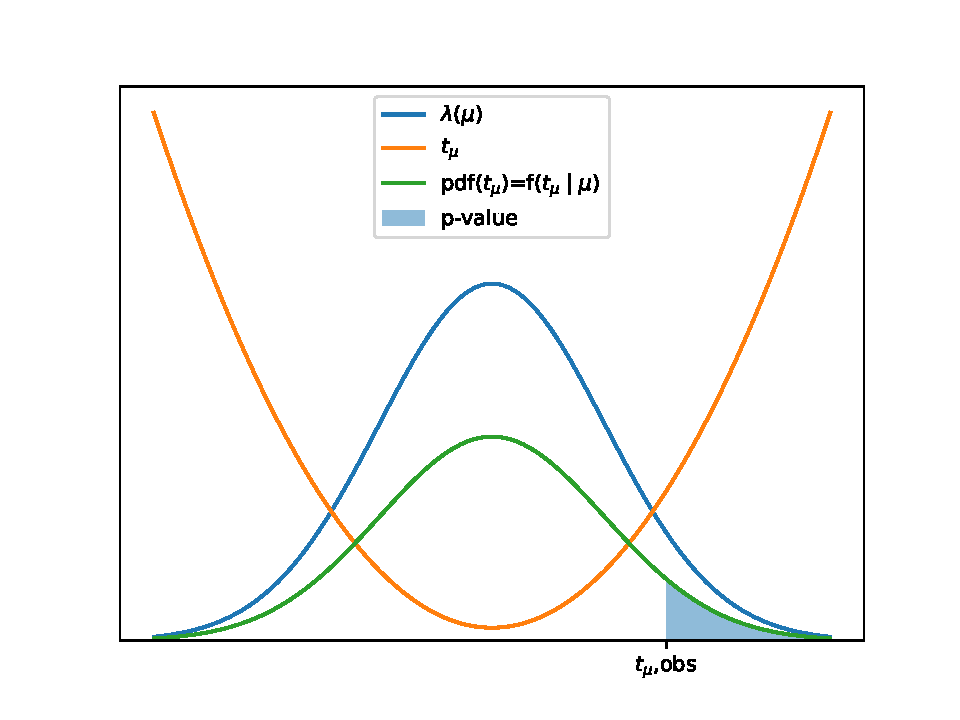
\includegraphics[width=0.7\textwidth]{test_stat_example.pdf}
        \caption[]{This is a sketch to mentally trace the transformation steps. The profile likelihood has essentially a hill like form with a maximum at ${\lambda(\hat{\mu},\hat{\bm{\Theta}})}$, $t_\mu$ is $\sim \mathrm{-ln}(\lambda)$ and under the assumption that the Poissonian model is correct the pdf of $t_\mu$ should peak at ${\lambda(\hat{\mu},\hat{\bm{\Theta}})}$}
    \label{fig:test_stat_example}    
\end{figure}

\subsection{The CL$_s$ value}\label{sec:cls}
Being able to calculate p-values allows now to state how likely it is that the proposed hypothesis is reflected by the observed data. Taking the example from the sketch in fig. \ref{fig:test_stat_example} one sees that the blue shaded area makes up about $\sim$\SI{10}{\percent} of the total area below the curve of $f(t_\mu \mid \mu)$. Since $f(t_\mu \mid \mu)$ is a pdf it holds that $\int f(t_\mu \mid \mu) =1$ and therefore gives a p-value of $p\sim 0.1$. With other words it means if we were to repeat the experiment, in $\sim$\SI{10}{\percent} of the cases the observed data would be in agreement with our proposed hypothesis. 

Particle physicists are usually interested in two things when making statistical tests for discovery of new phenomena: how well is the modeling of backgrounds (things we know) and can we find evidence in the observations for a new phenomenon. This means one needs to test two hypotheses: a background only ($b$) and a signal plus background ($s+b$) hypothesis. Each will result in a p-value on their own. For example $p_{b}=1$ would mean that the backgrounds are perfectly reflected by the observations and a $p_{s+b} < 0.05$ could be a sign of new physics. To combine these two metrics into a single score particle physicists came up with the pseudo Confidence Level called CL$_s$ incorporating also the goodness of the modeling of the backgrounds 
\begin{equation}
    \mathrm{CL}_s=\frac{\mathrm{CL}_{s+b}}{\mathrm{CL}_{b}}=
    \frac
    {\int_{t_{\mu=1 ,obs}}^{\infty} 
    f(t_\mu \mid \mu=1) \mathrm{d}t_\mu}
    {\int_{t_{\mu=0 ,obs}}^{\infty} 
    f(t_\mu \mid \mu=0) \mathrm{d}t_\mu}.
\end{equation}
This can also be understood visually from the first figure of the heavily cited CL$_s$ paper \citep{read2002presentation} (fig. \ref{fig:cls}). The left figure depicts the pdf's of the test statistic $ f(t_\mu \mid \mu=0)$ of the signal + background ({\color[HTML]{804000}{$\diagup$}}) and background ({\color[HTML]{2100FF}{$\diagup$}}) only hypotheses. The p-value is calculated by integration from $t_{\mu,obs}$ (the red observed line ({\color[HTML]{FF0000}{$\diagup$}})) to infinity (see eq. \ref{eq:p-value}). The green shaded area (\hexbox{00FF00}) corresponds to $p_{s+b}$ whereas the integral from the red line to infinity for the blue curve would be $p_b$. 

The right hand side depicts the degradation of search sensitivity (a)->(c). Unfortunately the colors of the pdf's changed here to signal + background (\hexbox{2100FF}) and background only (\hexbox{FF0000}). For example if you put the observation on the x-axis at 0 in these plots, you would get for the first one basically $p_{b}\approx 1$ and $p_{s+b}\approx 0$ resulting in a CL$_s\approx 0$, whereas with increasing overlap the CL$_s$ value increases and the sensitivity decrease.

\begin{figure}
    \centering
    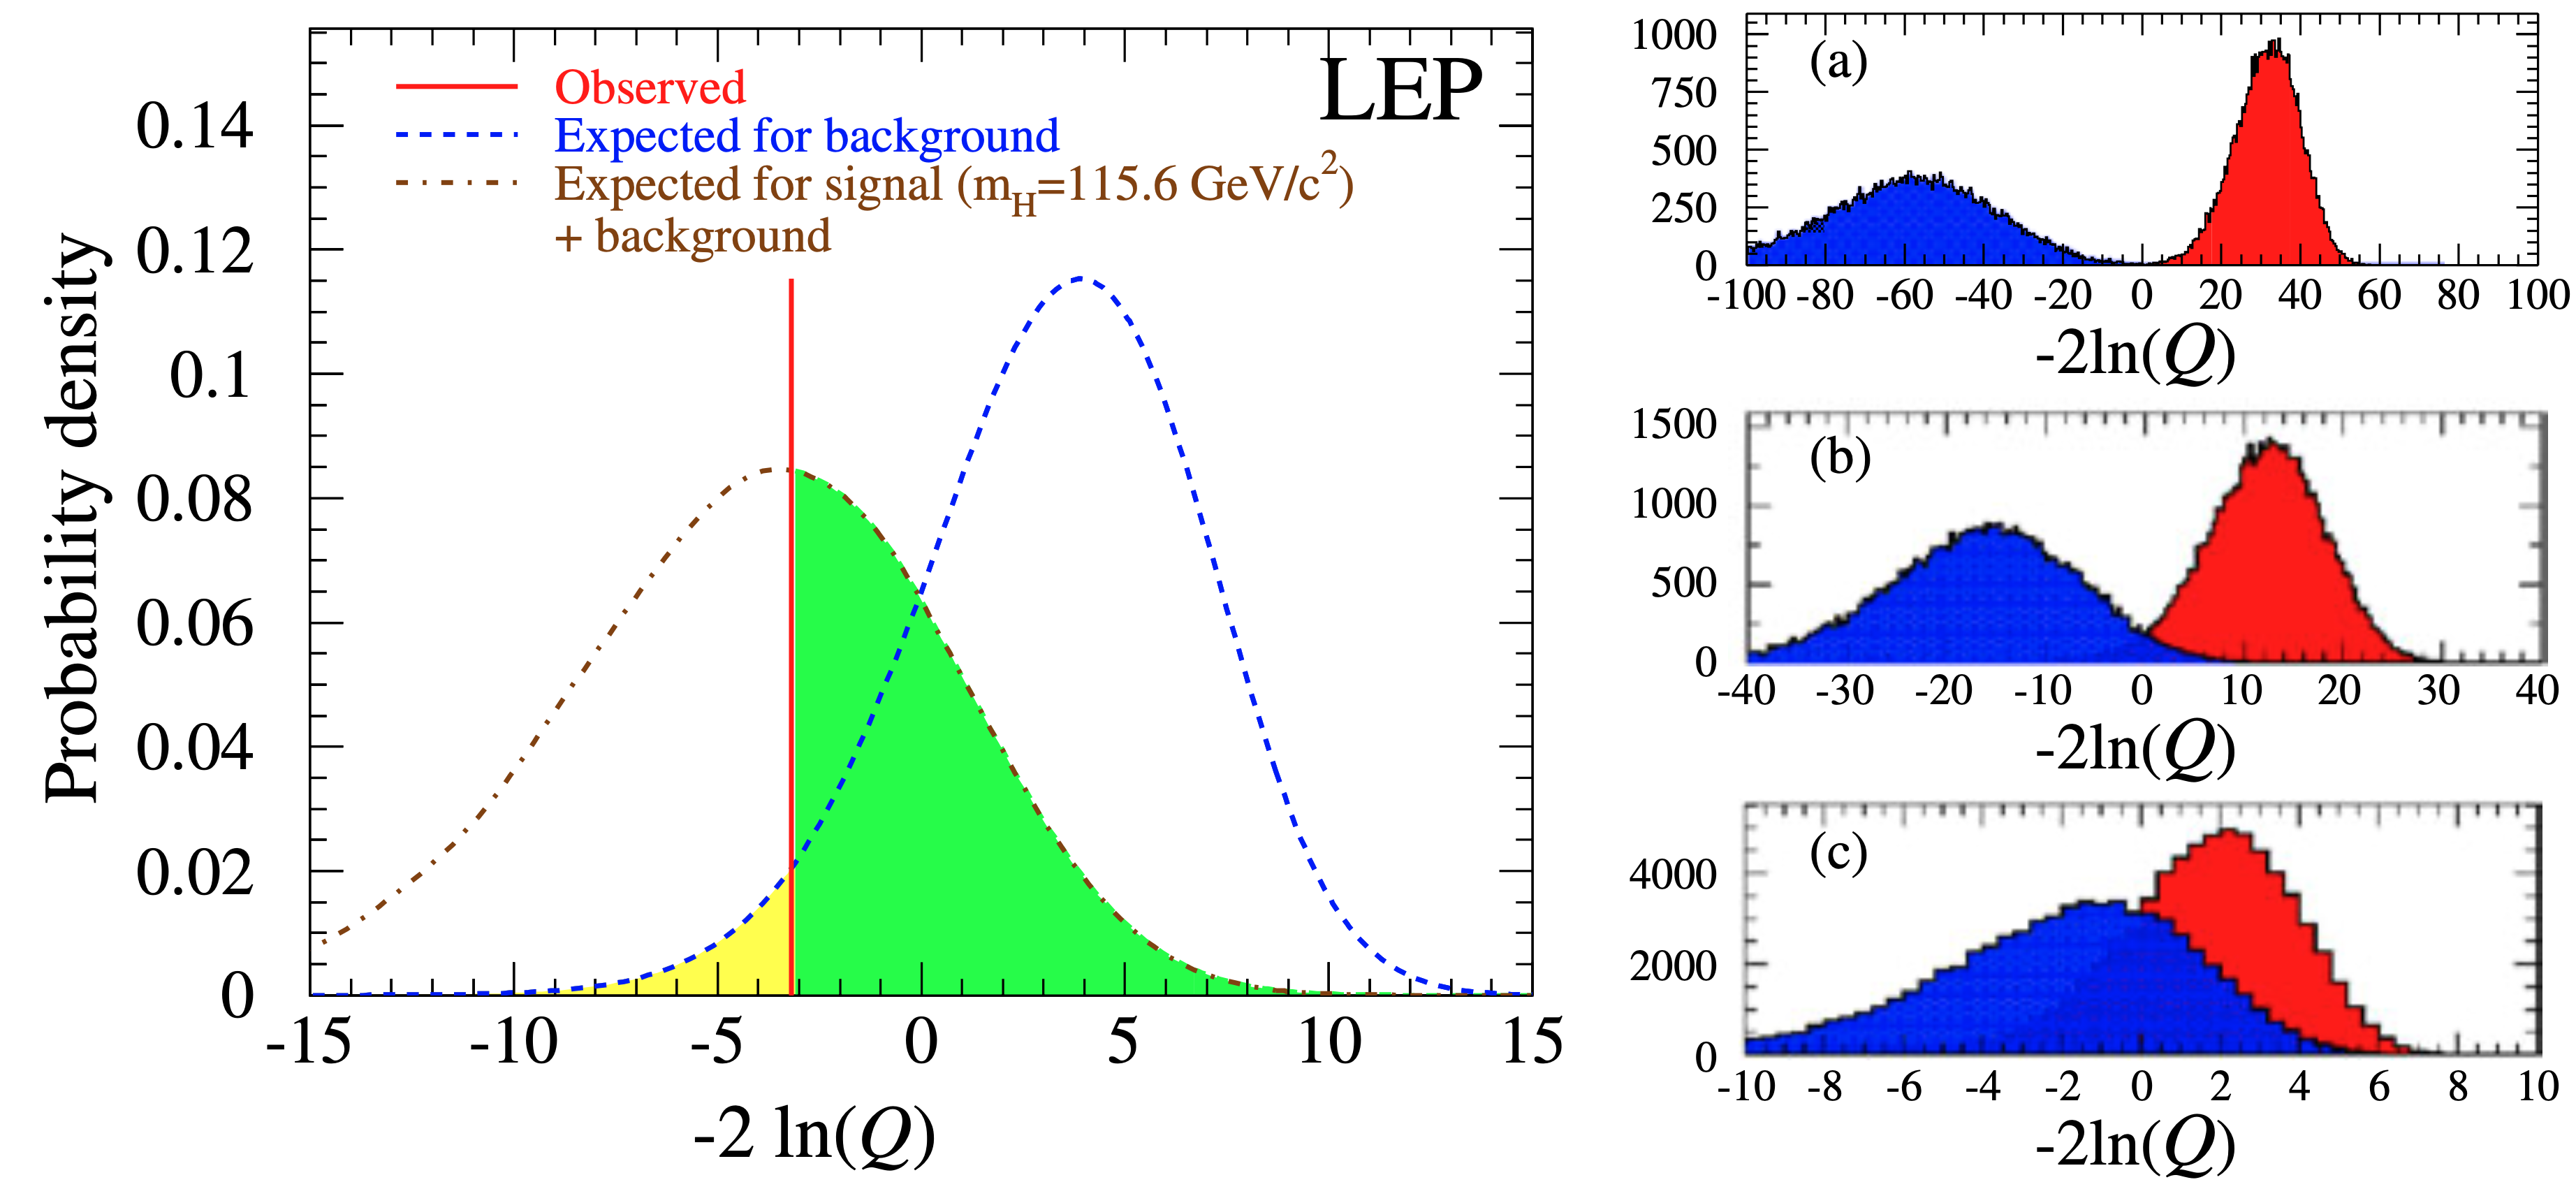
\includegraphics[width=1\textwidth]{cls.png}
        \caption[]{Probability density functions of test statistics from a Higgs search at LEP illustrating the calculation of p-values. Description at the end of section \ref{sec:cls}. From \citep{read2002presentation}.}
    \label{fig:cls}    
\end{figure}



\subsection{Histfactory in pyhf}



Detector-simulation related uncertainty
– Calibrations (electron, jet energy scale)
– Efficiencies (particle ID, reconstruction)
– Resolutions (jet energy, muon momentum)!
!
• Theoretical uncertainties
– Factorization/Normalization scale of MC generators
– Choice of MC generator (ME and/or PS, e.g. Herwig vs Pythia)
• Monte Carlo Statistical uncertainties
– Statistical uncertainty of simulated samples

